% Modelo de Trabalho Acadêmico da UNESP - Preenchido (Parte 1)

\PassOptionsToPackage{colorlinks=true, allcolors=black}{hyperref}
\documentclass[
  12pt,		
  a4paper,	
  openright,  
  oneside,	
  chapter=TITLE,		
  section=TITLE,		
  english,	
  french,	    
  spanish,	
  brazil	    
]{abntex2}

%----------------------------------------------------------------------------------------%
% P A C O T E S
%----------------------------------------------------------------------------------------%
    \usepackage{pacoteBasico}   
    \usepackage{color}		    
    \usepackage{graphicx}	    
    \usepackage{lipsum}		    
    \usepackage{pdfpages}       
    \usepackage[table,xcdraw]{xcolor}
    \usepackage{tikz}
    \usetikzlibrary{positioning, arrows.meta, shapes.geometric}
    \pgfdeclarelayer{background}
    \pgfsetlayers{background,main}
    
%----------------------------------------------------------------------------------------%
% I N F O R M A Ç Õ E S   B Á S I C A S   S O B R E   O   T R A B A L H O
%----------------------------------------------------------------------------------------%
    \newcommand{\nomeDoAutor}{Gabriel Martins Brum}
    \newcommand{\nomeDoCurso}{Ciências da Computação} % Ajuste se for outro curso
    \newcommand{\tituloDoTrabalho}{Classificação de Imagens Médicas via Fusão de Deep Learning e Redes Complexas utilizando Redes Neurais Recorrentes}
    \newcommand{\subtituloDoTrabalho}{}
    \newcommand{\tipoDeTrabalho}{Trabalho de Conclusão de Curso}
    \newcommand{\NomeDaFaculdade}{Instituto de Biociências, Letras e Ciências Exatas}
    \newcommand{\GrauAcademico}{Bacharelado} % Ajuste se for outro grau
    \newcommand{\AreaDeConcentracao}{Ciência da Computação} % Ajuste se for outra área
    \newcommand{\dataDeDefesa}{dd/mm/yyyy} % Substitua pela data real
    \newcommand{\anoDeEntrega}{2026}
    
%----------------------------------------------------------------------------------------%
% D A D O S   D O S   O R I E N T A D O R E S,   B A N C A   E   C O O R D E N A D O R
%----------------------------------------------------------------------------------------%
    \newcommand{\nomeDoOrientador}{Leandro Alves Neves}
    \newcommand{\tituloDoOrientador}{Prof. Dr.}
    \newcommand{\NomeDoCoorientador}{}
    \newcommand{\tituloDoCoorientador}{}
    \newcommand{\instituicaoorientador}{UNESP - IBILCE}     
    \newcommand{\instituicaocoorientador}{}
   
    % Preencha com os nomes reais dos membros da banca quando tiver
    \newcommand{\nomeDoMembroA}{Wallace Correa de Oliveira Casaca}
    \newcommand{\tituloDoMembroA}{Prof. Dr.}
    \newcommand{\instituicaomembroA}{UNESP - IBILCE}
    
    \newcommand{\nomeDoMembroB}{Guilherme Freire Roberto}
    \newcommand{\tituloDoMembroB}{Prof. Dr.}
    \newcommand{\instituicaomembroB}{UNESP - IBILCE}
    
    \newcommand{\nomeDoMembroC}{}
    \newcommand{\tituloDoMembroC}{}
    \newcommand{\instituicaomembroC}{}
    
    \newcommand{\nomeDoMembroD}{}
    \newcommand{\tituloDoMembroD}{}
    \newcommand{\instituicaomembroD}{}

%----------------------------------------------------------------------------------------%
% D A D O S   D A   I N S T I T U I Ç Ã O
%----------------------------------------------------------------------------------------%
    \newcommand{\nomeDaCidade}{São José do Rio Preto - SP}
    \newcommand{\nomeDaUniversidade}{
    Universidade Estadual Paulista -- UNESP\\
    \NomeDaFaculdade -- Campus de\ \nomeDaCidade
    }

%----------------------------------------------------------------------------------------%
% I N Í C I O   D O   D O C U M E N T O - P R É   T E X T U A L
%----------------------------------------------------------------------------------------%
\begin{document}
    
    \imprimircapa
    \imprimirfolhaderosto
    
    % F O L H A   D E   A P R O V A Ç Ã O
    \begin{folhadeaprovacao}
        \begin{center}
        \normalsize{\textbf{\MakeUppercase\nomeDoAutor}}
        \\
        \vspace*{1cm}
        \normalsize{\textbf{\MakeUppercase\tituloDoTrabalho}}
        \\
        \subtituloDoTrabalho
        \end{center}
                
        \vspace*{2cm}
        
        \noindent\tipoDeTrabalho\ apresentado(a) à Universidade Estadual Paulista (UNESP),\ \NomeDaFaculdade,\ \nomeDaCidade, para obtenção do título de\ \GrauAcademico{ }em\ \nomeDoCurso.
        \par
        \vspace*{1cm} 
        \noindent {Área de Concentração: \AreaDeConcentracao}
        \vspace*{1cm} 
       
       \noindent Data de defesa: \dataDeDefesa
        \vspace*{1cm}
       
       \noindent{BANCA EXAMINADORA}
       \vspace*{1cm}
       
       \raggedright\makebox[2.5in]{\hrulefill}\\
       \tituloDoOrientador \nomeDoOrientador \\ \instituicaoorientador
       \vspace*{1cm}
       
       \raggedright\makebox[2.5in]{\hrulefill}\\
       \tituloDoMembroA\ \nomeDoMembroA \\ \instituicaomembroA
       \vspace*{1cm}
       
       \raggedright\makebox[2.5in]{\hrulefill}\\
       \tituloDoMembroB\ \nomeDoMembroB \par \instituicaomembroB
       \vspace*{1cm}
       
       % Se houver mais membros, descomente as linhas abaixo
       % \raggedright\makebox[2.5in]{\hrulefill}\\
       % \tituloDoMembroC\ \nomeDoMembroC \\ \instituicaomembroC
       % \vspace*{1cm}
       
       % \raggedright\makebox[2.5in]{\hrulefill}\\
       % \tituloDoMembroD\ \nomeDoMembroD \\ \instituicaomembroD
       
    \end{folhadeaprovacao}
    
    % D E D I C A T Ó R I A
    \begin{dedicatoria}
        \vspace*{\fill}
        \begin{flushright}
            Aos meus pais e namorada, pelo apoio e incentivo durante toda a graduação.\\ % Exemplo
        \end{flushright}
        \vspace*{1cm}
    \end{dedicatoria}

    % A G R A D E C I M E N T O S
    \begin{agradecimentos}
        Gostaria de agradecer ao Prof. Dr. Leandro Alves Neves pela orientação... % Exemplo
    \end{agradecimentos}
    
    % E P Í G R A F E
    \begin{epigrafe}
        \vspace*{\fill}
    	\begin{flushright}
    		\textit{
        		"Presentemente, eu posso me considerar um sujeito de sorte\\
                Porque apesar de muito moço, me sinto são, e salvo, e forte"\\
                (Belchior)
            }
    	\end{flushright}
    \end{epigrafe}
    
    % R E S U M O
    \begin{resumo}
        O avanço das arquiteturas de aprendizado profundo revolucionou a análise computacional... % Começaremos a escrever aqui depois
        
        \vspace*{0.5cm}
        \noindent\textbf{{Palavras-Chave: }} Redes Complexas; Redes Neurais Recorrentes; Classificação de Imagens Médicas; Fusão Tardia; Deep Learning.
    \end{resumo}
    
    % A B S T R A C T
    \begin{resumo}[Abstract]
        The advancement of deep learning architectures has revolutionized computational analysis... % Começaremos a escrever aqui depois
        
        \vspace*{0.5cm}
        \noindent\textbf{{Keywords: }} Complex Networks; Recurrent Neural Networks; Medical Image Classification; Late Fusion; Deep Learning.
    \end{resumo}
    
    % L I S T A S
    \listoffigures*
    \newpage
    
    \listoftables*
    \newpage
    
    % Siglas descomentadas com exemplos relacionados ao seu TCC
    \begin{siglas}
        \item [CNN] \textit{Convolutional Neural Network} (Rede Neural Convolucional)
        \item [RNN] \textit{Recurrent Neural Network} (Rede Neural Recorrente)
        \item [RGB] \textit{Red, Green, Blue}
        \item [ViT] \textit{Vision Transformer}
    \end{siglas}  

    % Símbolos descomentados com exemplos relacionados ao seu TCC
    \begin{simbolos}
        \item[$r$] Raio de conexão do grafo
        \item[$k$] Número de partições na validação cruzada (k-Fold)
    \end{simbolos}
    
    % S U M Á R I O
    \tableofcontents*
    \newpage
    
    %------------------------------------------------------------------------------------%
    % C O R P O   D O   T E X T O
    %------------------------------------------------------------------------------------%
    \textual
    \pagestyle{simple} 
    
    % Classificação de Imagens Médicas via Fusão de Deep Learning e Redes Complexas utilizando Redes Neurais Recorrentes

    \chapter{Introdução}
    % classificação de imagens médicas + feature extraction + redes complexas + rnn + late fusion + hybrid models

    % motivações e justificativas?

    \chapter{Objetivos}
    % chapter de objetivos com questão de pesquisa e hipóteses?
    
    % \chapter{Revisão Bibliográfica}
    

    \chapter{Fundamentação Teórica}
    % % feature extraction in medical images + complet networks applications + recurrent neural networks gerando embedding topológico  + hybrid models gerando embedding topolico + late fusion via mlp

    \chapter{Metodologia}
    % Inicie a metodologia aqui...

    \begin{figure}[!hbtp]
    \centering
    % Escala em 80% para garantir que cabe bem na página do TCC
    \resizebox{0.80\columnwidth}{!}{%
    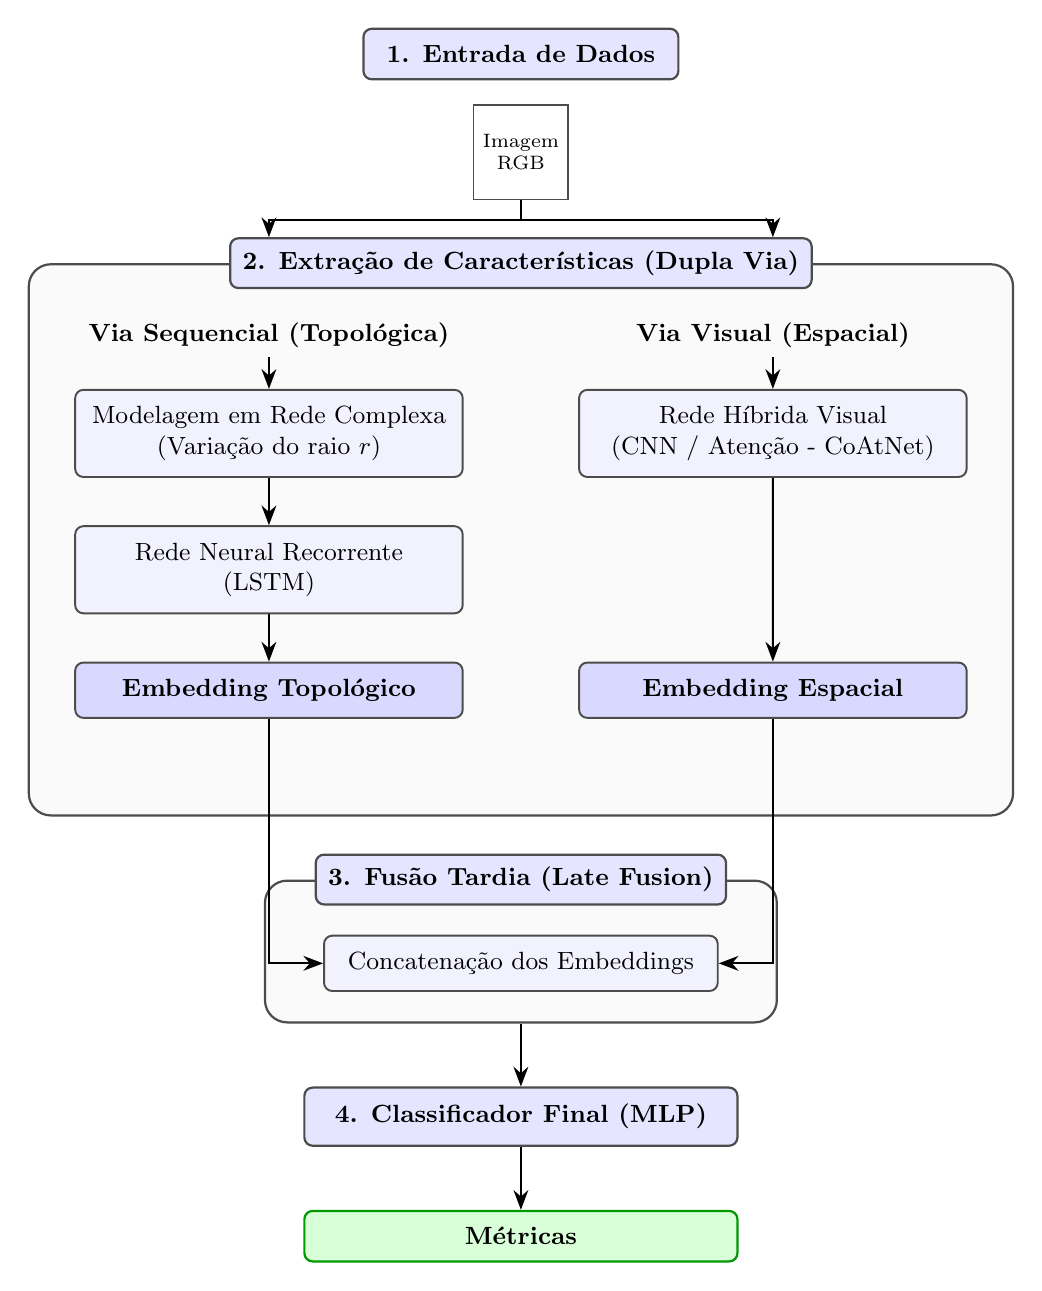
\begin{tikzpicture}[
        % Estilos
        recntagle/.style={
            rectangle, rounded corners=3pt, inner sep=6pt, align=center,
            font=\small\bfseries, draw=black!70, fill=blue!10, line width=0.8pt
        },
        title_block/.style={
            rectangle, rounded corners=3pt, inner sep=4.5pt, align=center,
            font=\small\bfseries, draw=black!70, fill=blue!10, line width=0.8pt
        },
        arrow/.style = {
            thick, ->, >={Stealth[length=2.5mm]}
        },
        box_delimitador/.style = {
            rectangle, rounded corners=8pt, draw=black!70, fill=black!2, line width=0.8pt
        },
        sub_block/.style = {
            rectangle, rounded corners=3pt, inner sep=6pt, align=center,
            draw=black!70, fill=blue!5, line width=0.7pt, font=\small
        },
        embed_block/.style = {
            rectangle, rounded corners=3pt, inner sep=6pt, align=center,
            draw=black!70, fill=blue!15, line width=0.7pt, font=\small\bfseries
        },
        img_node/.style = {
            rectangle, minimum size=1.2cm, draw=black!70, fill=white,
            line width=0.6pt, inner sep=2pt, align=center, font=\scriptsize
        }
    ]

        % 1. Entrada de Dados
        \node (input) [recntagle, minimum width=4cm] {1. Entrada de Dados};
        \node (input_img) [img_node, below=0.3cm of input] {Imagem\\RGB}; 
        
        % 2. CAIXA DA DUPLA VIA
        \node (twostream_box) [box_delimitador, minimum width=12.5cm, minimum height=7cm, below=0.8cm of input_img] {};
        \node (twostream_title) [title_block] at (twostream_box.north) {2. Extração de Características (Dupla Via)};

        % Títulos das vias
        \node (via_seq_title) [font=\bfseries\small] at ([xshift=-3.2cm, yshift=2.6cm]twostream_box.center) {Via Sequencial (Topológica)};
        \node (via_vis_title) [font=\bfseries\small] at ([xshift=3.2cm, yshift=2.6cm]twostream_box.center) {Via Visual (Espacial)};

        % Setas dividindo a entrada (AGORA PARAM NA BORDA SUPERIOR DA CAIXA)
        \draw [arrow] (input_img.south) -- ++(0,-0.25cm) -| ([xshift=-3.2cm]twostream_title.north);
        \draw [arrow] (input_img.south) -- ++(0,-0.25cm) -| ([xshift=3.2cm]twostream_title.north);

        % --- VIA SEQUENCIAL ---
        \node (complex_net) [sub_block, text width=4.5cm, below=0.4cm of via_seq_title] {Modelagem em Rede Complexa\\(Variação do raio $r$)};
        \node (rnn) [sub_block, text width=4.5cm, below=0.6cm of complex_net] {Rede Neural Recorrente\\(LSTM)};
        \node (embed_top) [embed_block, text width=4.5cm, below=0.6cm of rnn] {Embedding Topológico};

        \draw [arrow] (via_seq_title.south) -- (complex_net.north);
        \draw [arrow] (complex_net.south) -- (rnn.north);
        \draw [arrow] (rnn.south) -- (embed_top.north);

        % --- VIA VISUAL ---
        \node (cnn) [sub_block, text width=4.5cm, below=0.4cm of via_vis_title] {Rede Híbrida Visual\\(CNN / Atenção - CoAtNet)};
        \node (embed_vis) [embed_block, text width=4.5cm] at ([xshift=6.4cm]embed_top.center) {Embedding Espacial};

        \draw [arrow] (via_vis_title.south) -- (cnn.north);
        \draw [arrow] (cnn.south) -- (embed_vis.north);

        % 3. CAIXA DE FUSÃO TARDIA
        \node (fusion_box) [box_delimitador, minimum width=6.5cm, minimum height=1.8cm, below=0.8cm of twostream_box] {};
        \node (fusion_title) [title_block] at (fusion_box.north) {3. Fusão Tardia (Late Fusion)};
        
        \node (concat) [sub_block, minimum width=5cm] at ([yshift=-0.15cm]fusion_box.center) {Concatenação dos Embeddings};

        % Setas ligando os embeddings à fusão
        \draw [arrow] (embed_top.south) |- (concat.west);
        \draw [arrow] (embed_vis.south) |- (concat.east);

        % 4. CLASSIFICADOR FINAL
        \node (classif) [recntagle, minimum width=5.5cm, below=0.8cm of fusion_box] {4. Classificador Final (MLP)};
        \node (output) [recntagle, fill=green!15, draw=green!60!black, minimum width=5.5cm, below=0.8cm of classif] {Métricas};

        \draw [arrow] (fusion_box.south) -- (classif.north);
        \draw [arrow] (classif.south) -- (output.north);

    \end{tikzpicture}%
    }
    \caption{Arquitetura proposta do modelo híbrido \textit{Two-Stream} para classificação de imagens médicas, integrando extração visual por CNN e extração de características topológicas em grafos via LSTM.}
    \label{fig:pipeline_tcc}
\end{figure}


    \chapter{Resultados e Discussão}
    % Inicie os resultados aqui...
                
    \chapter{Conclusão}
    % Inicie a conclusão do seu trabalho aqui...
   
    %------------------------------------------------------------------------------------%
    % P Ó S   T E X T U A L
    %------------------------------------------------------------------------------------%
    \postextual
    
    % R E F E R Ê N C I A S
    \bibliography{referencias}

    % GLOSSÁRIO (Opcional)
    % \clearpage
    % \chapter*{GLOSSÁRIO} \addcontentsline{toc}{chapter}{GLOSSÁRIO} 
    % \noindent\textbf{Termo:} Definição...

    % A P Ê N D I C E S (Opcional)
    % \begin{apendicesenv}
    %     \chapter{TÍTULO DO APÊNDICE}
    %     % Insira o conteúdo do apêndice aqui...
    % \end{apendicesenv}
    
    % A N E X O S (Opcional)
    % \begin{anexosenv}
    %     \chapter{TÍTULO DO ANEXO}
    %     % Exemplo de inclusão de PDF:
    %     % \includepdf[pages=-]{arquivo.pdf}
    % \end{anexosenv}
    
\end{document}